\date{}
\title{}
\date{}
\begin{document}
\begin{frame}
    \titlepage
\end{frame}

\begin{frame}
\frametitle{last time}
\begin{itemize}
\item TCP packet format
    \begin{itemize}
    \item two instances of sliding window protocol
    \item seq number = first byte number of this packet
        \begin{itemize}
        \item or first byte number of next data packet
        \end{itemize}
    \item ack number = 1 + last byte number (of other end) ack'd
    \item seq/ack sent regardless of whether data packet or not
    \end{itemize}
\item switched networks from multi-access
    \begin{itemize}
    \item will explain Ethernet frame format we'll see
    \end{itemize}
\end{itemize}
\end{frame}

\begin{frame}
\frametitle{common timeout bugs}
\end{frame}


\section{datagrams and Ethernet format}

\usetikzlibrary{patterns}

\begin{frame}{typically sent on Ethernet}
\begin{tikzpicture}
\tikzset{
    box/.style={draw,thick},
    label/.style={font=\small},
    label large/.style={},
    missing/.style={pattern=north west lines},
    start and end/.style={alt=<2>{fill=red!10,text=red}},
    type field/.style={alt=<3-4>{fill=red!10,text=red}},
    destination address/.style={alt=<5-6>{fill=red!10,text=red}},
    source address/.style={alt=<7>{fill=red!10,text=red}},
}
\draw[start and end,box] (4, 0) rectangle (12, -1)
    node[midway,label] {preamble + start marker};
\draw[source address,box] (0, -1) rectangle (6, -2)
    node[midway,label] {source MAC address};
\draw[destination address,box] (6, -1) rectangle (12, -2)
    node[midway,label] {destination MAC address};
\draw[type field,box] (0, -2) rectangle (2, -3)
    node[midway,label] {type};
\draw[box] (2, -2) -- (12, -2) -- (12, -4) -- (0, -4) -- (0, -3) -| cycle;
    \node[label large] at (6, -3) {data (for next layer)};
\begin{visibleenv}<8>
\draw[red,ultra thick] (2, -2) -- (2, -3);
\draw[box,red,ultra thick,fill=white] (4.5, -3) rectangle (11.5, -4) 
    node[midway,label] {sometimes extra stuff (``tags'')};
\end{visibleenv}
\draw[box] (0, -4) rectangle (4, -5) node[midway,label] {checksum};
\draw[start and end,box,missing] (4, -4) rectangle (12, -5)
    node[midway,label,fill=white] {`interpacket gap'};
\draw[start and end,box,missing] (0, -5) rectangle (4, -6);
\begin{visibleenv}<2>
\node[align=left,draw=red,ultra thick,fill=white] at (6, -3) {
    explicit start marker \\
    end indicated by `gap' between signals
};
\end{visibleenv}
\begin{visibleenv}<3>
\node[align=left,draw=red,ultra thick,fill=white] at (8, -3) {
    type field indicates which next layer in use \\
    often varies on frame-by-frame basis \\
};
\end{visibleenv}
\begin{visibleenv}<4>
\node[align=left,draw=red,ultra thick,fill=white] at (8, -3) {
    actually \texttt{type/length} for historical reasons \\
    but most commonly used for type these days
};
\end{visibleenv}
\begin{visibleenv}<5>
\node[align=left,draw=red,ultra thick,fill=white] at (6, -4) {
    destination address indicates who frame is for \\
    present regardless of whether switching is in use \\
    ~ \\
    each host \myemph{filters} out frames for `wrong' destination address
};
\end{visibleenv}
\begin{visibleenv}<6>
\node[align=left,draw=red,ultra thick,fill=white] at (6, -4) {
    since destination address always present \\
    as last resort, switches can send every frame to everyone \\
    ~ \\
    will still work, just much less efficient
};
\end{visibleenv}
\begin{visibleenv}<7>
\node[align=left,draw=red,ultra thick,fill=white] at (6, -4) {
    who the frame came from \\
    gives `return address' for sending replies \\
    ~ \\
    will also be used by switches
};
\end{visibleenv}
\end{tikzpicture}
\end{frame}

\begin{frame}{MAC addresses}
    \begin{itemize}
    \item MAC [media access control] addresses
    \item used by Ethernet, Wifi, and lots of other protocols
    \item 48-bit number written in hex: \texttt{01:23:45:67:89:AB}
        \begin{itemize}
        \item (sometimes seperated with \texttt{-} instead of \texttt{:})
        \end{itemize}
    \item assigned by IEEE to networking manufacturers in blocks
        \begin{itemize}
        \item Institution of Electrical and Electronics Engineers
        \item example: \texttt{00:02:B3:}\ldots, \texttt{00:03:47:}\ldots, (and many more) for Intel
        \end{itemize}
    \vspace{.5cm}
    \item individual addresses hard-coded in networking hardware
        \begin{itemize}
        \item uniquely identify port/device
        \end{itemize}
    \end{itemize}
\end{frame}

\begin{frame}{special MAC addresses}
    \begin{itemize}
    \item \texttt{00:00:00:00:00:00} (all zeroes)
    \item \texttt{FF:FF:FF:FF:FF:FF} (all ones), \texttt{FF:}\ldots
        \begin{itemize}
        \item special destination meaning ``send to everyone'' (on this network)
        \item called \textit{broadcast}
        \end{itemize}
    \item \texttt{01:80:C2:}\ldots, \texttt{33:33:}\ldots, (and some more)
        \begin{itemize}
        \item special destinations representing multiple receivers
        \item example: `all IPv6 routers on this network' (\texttt{33:33:00:00:00:02})
        \item called \textit{multicast}
        \end{itemize}
    \end{itemize}
\end{frame}

\begin{frame}{larger MAC addresses}
    \begin{itemize}
    \item IEEE now calls MAC address EUI-48 (48-bit Extended Unique Identifier)
    \vspace{.5cm}
    \item also created EUI-64, with 64-bit addresses
        \begin{itemize}
        \item way of mapping EUI-48s to EUI-64s
        \item turns out 48 bits might have been low
        \end{itemize}
    \item I'm not sure what status is on switching to 64-bit addresses
        \begin{itemize}
        \item IEEE 802.15.4 (used in ZigBee, 6LoWPAN, some others) uses EUI-64
        \item I don't know other local network protocols that do
        \end{itemize}
    \end{itemize}
\end{frame}


% FIXME: example in wireshark

\subsection{versus virtual circuits}

\begin{frame}{datagram idea}
    \begin{itemize}
    \item can always send something to anyone on network
        \begin{itemize}
        \item just put destination MAC in frame
        \end{itemize}
    \item no need for reservations/`connections'/etc.
        \begin{itemize}
        \item not like the interface you've seen with [TCP] sockets
        \end{itemize}
    \vspace{.5cm}
    \item not the only model for networks (and internetworks)
    \end{itemize}
\end{frame}

\begin{frame}{virtual circuit}
    \begin{itemize}
    \item other model: virtual circuit
    \item two machines setup a `circuit'
        \begin{itemize}
        \item some sort of `special' messages to do this
        \end{itemize}
    \item switches/routers \myemph{reserve resources} for circuit
        \begin{itemize}
        \item ``gaurenteed'' bandwidth
        \end{itemize}
    \item transmitted data must be part of estabished circuit
    \vspace{.5cm}
    \item example: ATM (Asynchronous Transfer Mode)
        \begin{itemize}
        \item used (?historically?) by some telephone networks
        \end{itemize}
    \end{itemize}
\end{frame}


\section{switch architecture}

\subsection{not programmable}
\begin{frame}{an annoyance}
    \begin{itemize}
    \item traditionally, switches/routers have been `fixed function' specialized hardware
    \vspace{.5cm}
    \item special hardware needed for multigigabit performance
    \item limited configuration options
    \item usually non-automated configuration
        \begin{itemize}
        \item login to each managed switch/router to change settings
        \item no standardization for configuration across vendors
        \end{itemize}
    \item little visibility into internal design
        \begin{itemize}
        \item even though switches/routers often running complicated programs
        \end{itemize}
    \end{itemize}
\end{frame}

\begin{frame}{the historical situation}
    \begin{itemize}
    \item let's say I want to design a new extension to Ethernet
    \vspace{.5cm}
    \item historical options if want to test/deploy it\ldots
        \begin{itemize}
        \item implement it in slow/low-capacity software/FPGA switch
        \vspace{.5cm}
        \item convince switch HW company to implement it
        \vspace{.5cm}
        \item contort extension to fit with features not intended for use case
            \begin{itemize}
            \item example: using VPN support to change path of frames on network
            \end{itemize}
        \end{itemize}
    \end{itemize}
\end{frame}



\subsection{control v dataplane}
\begin{frame}{software defined networking (SDN)}
    \begin{itemize}
    \item movement toward \textit{programmable} networks
    \vspace{.5cm}
    \item ``software-defined''
        \begin{itemize}
        \item rules about how network works defined in ``normal'' software
        \end{itemize}
    \end{itemize}
\end{frame}

\begin{frame}{control plane and data plane}
    \begin{itemize}
    \item control plane
        \begin{itemize}
        \item decides \textit{how} to handle traffic
        \item ``slow path'', where complicated decisions are
        \end{itemize}
    \item data plane
        \begin{itemize}
        \item actually implements the decisions made by the control plane
        \item ``fast path'', implementing simple rules
        \end{itemize}
    \vspace{.5cm}
    \item probably what switches did internally before SDN was a thing
    \end{itemize}
\end{frame}

\begin{frame}{separate control/data plane}
    \begin{itemize}
    \item one SDN key idea: separate control and data plane
    \item allow new \myemph<2>{vendor-neutral} implementations of control plane
        \begin{itemize}
        \item requires standard interface for programming data plane
        \item most prominent example: OpenFlow
        \end{itemize}
    \item easily allows for central `control plane' server
        \begin{itemize}
        \item instead of separate control plane running on each switch/router
        \end{itemize}
    \end{itemize}
\end{frame}


\subsection{what is P4}

\begin{frame}{P4}
    \begin{itemize}
    \item P4 --- programming langauge for data planes
    \item intended to be compiled to run on fast switches
    \item includes `runtime' defining how control plane configures data plane
    \end{itemize}
\end{frame}

\begin{frame}{future P4 assignment}
    \begin{itemize}
    \item given: 
        \begin{itemize}
        \item simple P4 switch that doesn't know where to direct frames
        \item simpler controller (in Python) that configures switch
        \item simulated 4-machine network in VM
        \end{itemize}
    \item your task will be:
        \begin{itemize}
        \item have controller write static configuration to direct to right place
        \item modify data plane to send information to control plane
        \item have controller change configuration based on info from data plane
        \end{itemize}
    \item (we'll discuss more details later)
    \end{itemize}
\end{frame}


\subsection{P4 dataplane}
\subsubsection{switch parts}
\usetikzlibrary{arrows.meta,decorations.pathreplacing}
\begin{frame}[fragile,label=p4arch]{P4 switch architecture}
\begin{tikzpicture}
\tikzset{
    queue/.style={alt=<2>{fill=red!10,draw=red,ultra thick}},
    explain box/.style={
        align=left,at={(explain box top)},anchor=north,draw=red,very thick
    },
}
\begin{scope}[x=.7cm]
\foreach \x in {1,2,3,4} {
    \node[anchor=east] at (0, \x-.5) {IN$\rightarrow$};
    \node[anchor=west] at (17.5, \x-.5) {$\rightarrow$OUT};
    \foreach \noff in {0,8,16} {
        \begin{scope}[shift={(\noff, 0)},yshift=\x cm-1cm,y=0.9cm]
            \draw[queue,thick] (0, 0) rectangle (1.5, 1);
            \foreach \off in {.5,.7,.9,1.1,1.3} {
                \draw[queue,thick] (\off, 0) -- (\off, 1);
            }
        \end{scope}
    }
}
\coordinate (explain box top) at (8.5, -.7);
\tikzset{
    box/.style={draw,thick},
    box label/.style={font=\fontsize{9}{10}\selectfont},
    parserBox/.style={alt=<6>{fill=red!10}},
    deparserBox/.style={alt=<7>{fill=red!10}},
    ingressBox/.style={alt=<8>{fill=red!10}},
    egressBox/.style={alt=<8>{fill=red!10}},
};
\foreach \x/\name in {2/parser,4/ingress,6/deparser} {
    \draw[box,\name Box] (\x, 0) coordinate (\name-in-base) rectangle ++(1.6, 4) coordinate (\name-in-other-base) node[midway,box label,alias=x] (\name-in-label) {\name};
    \coordinate (\name-in-bottom-right) at (\name-in-base);
    \coordinate (\name-in-bottom-left) at (\name-in-base -| \name-in-other-base);
    \draw[box] (\x + 1.4, -.1) |- (\x - .2, .8-1) |- (\x-.1, 3.8); 
    \draw[box] (\x + 1.5, 0) |- (\x - .1, .9-1) |- (\x, 3.9); 
}
\foreach \x/\name in {10/parser,12/egress,14/deparser} {
    \draw[box,\name Box] (\x, 0) coordinate (\name-out-base) rectangle ++(1.6, 4) coordinate (\name-out-other-base) node[midway,box label] (\name-out label) {\name};
    \coordinate (\name-out-bottom-right) at (\name-out-base);
    \coordinate (\name-out-bottom-left) at (\name-out-base -| \name-out-other-base);
    \draw[box] (\x + 1.4, -.1) |- (\x - .2, .8-1) |- (\x-.1, 3.8); 
    \draw[box] (\x + 1.5, 0) |- (\x - .1, .9-1) |- (\x, 3.9); 
}
\end{scope}
\begin{visibleenv}<2>
    \node[explain box] {
        queues of frames to be processed \\
        if needed, hold packets in between processing steps 
    };
\end{visibleenv}
\begin{visibleenv}<3>
    \foreach \x in {in,out} {
        \draw[line width=.5mm,red,decorate,decoration={brace,mirror,raise=3mm,amplitude=2mm}]
            ([xshift=-.2cm]parser-\x-bottom-right) --
            ([xshift=.2cm]deparser-\x-bottom-left);
    }
    \node[explain box] {
        \textit{ingress} and \textit{egress} pipelines
    };
\end{visibleenv}
\begin{visibleenv}<4>
    \foreach \x in {in} {
        \draw[line width=.5mm,red,decorate,decoration={brace,mirror,raise=3mm,amplitude=2mm}]
            ([xshift=-.2cm]parser-\x-bottom-right) --
            ([xshift=.2cm]deparser-\x-bottom-left);
    }
    \node[explain box] {
        ingress pipeline: processes every input frame \\
        primary job: decide where to forward frame (if anywhere) 
    };
\end{visibleenv}
\begin{visibleenv}<5>
    \foreach \x in {out} {
        \draw[line width=.5mm,red,decorate,decoration={brace,mirror,raise=3mm,amplitude=2mm}]
            ([xshift=-.2cm]parser-\x-bottom-right) --
            ([xshift=.2cm]deparser-\x-bottom-left);
    }
    \node[explain box] {
        egress pipeline: process every output frame \\
        run one time for \myemph{each copy} output
    };
\end{visibleenv}
\begin{visibleenv}<6>
    \foreach \x in {in,out} {
        \draw[line width=.5mm,red,decorate,decoration={brace,mirror,raise=3mm,amplitude=2mm}]
            ([xshift=-.2cm]parser-\x-bottom-right) --
            ([xshift=.2cm]parser-\x-bottom-left);
    }
    \node[explain box] {
        parser: decode frame fields into temporary storage
    };
\end{visibleenv}
\begin{visibleenv}<7>
    \foreach \x in {in,out} {
        \draw[line width=.5mm,red,decorate,decoration={brace,mirror,raise=3mm,amplitude=2mm}]
            ([xshift=-.2cm]deparser-\x-bottom-right) --
            ([xshift=.2cm]deparser-\x-bottom-left);
    }
    \node[explain box] {
        deparser: converted decoded fields back into bytes for network
    };
\end{visibleenv}
\begin{visibleenv}<8>
    \foreach \x in {ingress-in,egress-out} {
        \draw[line width=.5mm,red,decorate,decoration={brace,mirror,raise=3mm,amplitude=2mm}]
            ([xshift=-.2cm]\x-bottom-right) --
            ([xshift=.2cm]\x-bottom-left);
    }
    \node[explain box] {
        ``match/action pipelines'' \\
        do series of table lookups based on parsed fields \\
        each table lookup specifies next action
    };
\end{visibleenv}
\end{tikzpicture}
\end{frame}

\begin{frame}[fragile]{P4: switch parts}
\begin{Verbatim}
V1Switch(
MyParser(),
MyVerifyChecksum(),
MyIngress(),
MyEgress(),
MyComputeChecksum(),
MyDeparser()
) main;
\end{Verbatim}
\begin{itemize}
\item code to declare instance of dataplane from functions for each part
\item will look at most of these components
    \begin{itemize}
    \item won't have reason to change verify/compute checksum
    \end{itemize}
\end{itemize}
\end{frame}

\subsubsection{header management}
\usetikzlibrary{arrows.meta,decorations.pathreplacing}


\begin{frame}[fragile]{P4: declaring headers (1)}
\providecommand{\vemphA}[1]{\myemph<2>{#1}}
\providecommand{\vemphB}[1]{\myemph<3>{#1}}
\providecommand{\vemphC}[1]{\myemph<4>{#1}}
\providecommand{\vemphD}[1]{\myemph<5>{#1}}
\begin{Verbatim}[fontsize=\small,commandchars=\\@~]
typedef bit<48> macAddr_t;
\vemphA@@header~ ethernet_t~ {
    macAddr_t srcAddr;
    macAddr_T dstAddr;
    bit<16>   etherType;
}
\end{Verbatim}
\begin{itemize}
\item<2-> kinda like \Verb|typedef struct { ... } ethernet_t;|
\item<3-> order needs to \textit{exactly} match what's sent on network
    \begin{itemize}
    \item switch will do bit-by-bit copy into this struct
    \end{itemize}
\end{itemize}
\end{frame}

\begin{frame}[fragile]{P4: declaring headers (2)}
\providecommand{\vemphA}[1]{\myemph<2>{#1}}
\providecommand{\vemphB}[1]{\myemph<3>{#1}}
\providecommand{\vemphC}[1]{\myemph<4>{#1}}
\providecommand{\vemphD}[1]{\myemph<5>{#1}}
\begin{Verbatim}[fontsize=\small,commandchars=\\@~]
\vemphA@struct headers~ {
    \vemphB@ethernet_t~   ethernet;
    \vemphB@ipv4_t~       ipv4;
    \vemphB@ipv6_t~       ipv6;
}
\end{Verbatim}
\begin{itemize}
\item<2-> struct of all possible headers
    \begin{itemize}
    \item from all layers the switch/router handles
    \item not all frames will use all of them, some may be mutually exclusive
    \item order does not need to match frame storage (will write code to handle that)
    \end{itemize}
\item<3-> references header types defined previously
\end{itemize}
\end{frame}

% FIXME: hilite parts with explanation
\begin{frame}[fragile]{P4: parsing}
\begin{Verbatim}
parser MyParser(
    packet_in packet,
    out headers hdr,
    inout metadata meta,
    inout standard_metadata_t standard_metadata) {
\end{Verbatim}
\begin{itemize}
\item function modifies `out' parameters instead of returning
\item parser function --- takes parameters:
    \begin{itemize}
    \item packet --- the input frame
    \item headers --- extracted headers (\texttt{struct headers})
    \item meta --- program's local variables about frame (\texttt{struct metadata})
    \item standard\_metadata --- info for system about frame
        \begin{itemize}
        \item where frame came from, where it should go, etc.
        \end{itemize}
    \end{itemize}
\end{itemize}
\end{frame}

\begin{frame}[fragile]{P4: parsing}
\providecommand{\vemphA}[1]{\myemph<2>{#1}}
\providecommand{\vemphB}[1]{\myemph<3>{#1}}
\providecommand{\vemphC}[1]{\myemph<4>{#1}}
\providecommand{\vemphD}[1]{\myemph<5>{#1}}
\begin{Verbatim}[fontsize=\small,commandchars=\\@~]
parser MyParser(...) {
    \vemphA@state~ start {
        \vemphB@transition~ \vemphC@parse_ethernet~;
    }
    \vemphA@state~ \vemphC@parse_ethernet~ {
        \vemphD@packet.extract(hdr.ethernet);~
        \vemphB@transition~ select(hdr.ethernet.etherType) {
            TYPE_IPV4: parse_ipv4;
            TYPE_IPV6: parse_ipv6
            default: accept;
        }
    }
    ....
}
\end{Verbatim}
\begin{tikzpicture}[overlay,remember picture]
    \begin{visibleenv}<2>
    \node[align=left,draw=red,fill=white,very thick] at (current page.center) {
        functions written as state machine \\
        exectuion starts in state \texttt{start} \\
        follows instructions in each state
    };
    \end{visibleenv}
    \begin{visibleenv}<3-4>
    \node[align=left,draw=red,fill=white,very thick] at ([yshift=-1cm]current page.center) {
        transition statements say which state to go to next  \\
        can be conditional using switch-statement-like syntax
    };
    \end{visibleenv}
    \begin{visibleenv}<5>
    \node[align=left,draw=red,fill=white,very thick] at ([yshift=-1.5cm]current page.center) {
        \texttt{extract} operation copies from packet \\
        into specific \texttt{header} object
    };
    \end{visibleenv}
\end{tikzpicture}
\end{frame}

\subsubsection{exercise}
\begin{frame}{exercise: header representation (1)}
    \begin{itemize}
    \item let's say packet format is:
        \begin{itemize}
        \item 16 bit source address
        \item 16 bit destination address
        \item 1 bit flag ``is timestamp present''
        \item 1 bit flag ``is data present'
        \item 6 bits unused
        \item (optional) 32-bit timestamp
        \item (optional) 16-bit data size
        \item (optional) data
        \end{itemize}
    \item how to represent this?
        \begin{itemize}
        \item how many structs?
        \item what's in the \texttt{header \{\ldots\}}?
        \end{itemize}
    \end{itemize}
\end{frame}

\begin{frame}{}
\end{frame}

\begin{frame}[fragile]{exercise: header parsing}
\begin{Verbatim}[fontsize=\small]
struct basic_hdr_t {
    bit<16> src; bit<16> dst;
    bit<1> has_timestamp; bit<1> has_data; bit<6> unused;
};
struct timestamp_t {
    bit<32> timestamp;
}
struct data_hdr_t {
    bit<16> size;
}
\end{Verbatim}
\begin{itemize}
\item what states/transitions in parser?
\end{itemize}
\end{frame}

\begin{frame}[fragile]{states/transitions}
\begin{itemize}
\item parse\_basic:
    \begin{itemize}
    \item has\_timestamp: to parse\_timestamp:
    \item has\_data: to parse\_data
    \item otherwise: accept
    \end{itemize}
\item parse\_timestamp:
    \begin{itemize}
    \item has\_data: to parse\_data:
    \item otherwise: accept
    \end{itemize}
\item parse\_data: then accept
\end{itemize}
\end{frame}

\subsubsection{ingress processing}
\usetikzlibrary{arrows.meta,decorations.pathreplacing}


\begin{frame}[fragile]{P4: ingress processing}
\providecommand{\vemphA}[1]{\myemph<2>{#1}}
\providecommand{\vemphB}[1]{\myemph<3>{#1}}
\providecommand{\vemphC}[1]{\myemph<4>{#1}}
\providecommand{\vemphD}[1]{\myemph<5>{#1}}
\begin{itemize}
\item example: send \textit{everything} to output port number 4
\end{itemize}
\begin{Verbatim}[fontsize=\small,commandchars=\\@~]
control MyIngress(...) {
    apply {
        \vemphA@standard_metadata.egress_spec = 4;~
    }
}
\end{Verbatim}
\begin{tikzpicture}[overlay,remember picture]
    \begin{visibleenv}<2>
    \node[align=left,draw=red,fill=white,ultra thick] at ([yshift=-2cm]current page.center) {
        standard\_metadata --- `hard-coded' phase reads \texttt{egress\_spec} \\
        ~ \\
        special \texttt{egress\_spec} value for ``discard frame''
    };
    \end{visibleenv}
\end{tikzpicture}
\end{frame}

\begin{frame}{switch decisions}
    \begin{itemize}
    \item most decisions switches/routers make are table lookups
    \vspace{.5cm}
    \item take field from packet (e.g. destination)
    \item lookup in table what to do with that
        (e.g. send to port X, throw error, etc.)
    \vspace{.5cm}
    \item P4 has special syntax for tables and table lookups
    \end{itemize}
\end{frame}

\begin{frame}[fragile]{P4: tables}
\providecommand{\vemphA}[1]{\myemph<2>{#1}}
\providecommand{\vemphB}[1]{\myemph<3>{#1}}
\providecommand{\vemphC}[1]{\myemph<4>{#1}}
\providecommand{\vemphD}[1]{\myemph<5>{#1}}
\begin{Verbatim}[fontsize=\small,commandchars=\\@~]
\vemphA@table~ mac_dst_exact {
    \vemphB@key~ = {
        \vemphB@hdr.ethernet.dstAddr~ : \vemphC@exact~;
    }
    \vemphB@actions~ = {
        drop,
        forward_to,
    }
    size = 1024;
    default_action = drop();
}
\end{Verbatim}
\begin{tikzpicture}[overlay,remember picture]
\tikzset{
    box/.style={
        align=left,
        draw=red,
        fill=white,
        ultra thick,
        anchor=west,
        at={([xshift=1cm]current page.center)},
    },
}
    \begin{visibleenv}<2>
    \node[box] {
        declare a table with a name \\
        done has part of ingress/outgress
    };
    \end{visibleenv}
    \begin{visibleenv}<3>
    \node[box] {
        key/value structure \\
        keys usually from headers \\
        values are actions to run
    };
    \end{visibleenv}
    \begin{visibleenv}<4>
    \node[box] {
        here, each table entry \\
        contains whole address \\
        P4 also supports \\
        partially matched keys
    };
    \end{visibleenv}
\end{tikzpicture}
\end{frame}

\begin{frame}{P4 table key types}
    \begin{itemize}
    \item exact --- full entry
    \item lpm --- longest prefix match
        \begin{itemize}
        \item table entries contain `prefixes' of header field(s)
        \item we'll see motivation for this when we talk about routing
        \item if multiple entries match, take longest one
        \end{itemize}
    \item ternary --- 0/1/don't care
        \begin{itemize}
        \item table entries contain key and mask
        \item entry matches if bits included in mask match
        \item other view: keys represented with 0/1/don't care `trits'
        \end{itemize}
    \end{itemize}
\end{frame}

\begin{frame}{content-addressable memory}
    \begin{itemize}
    \item high-end routers/switches have \textit{content addressable memory} (CAM)
    \item \ldots including \textit{ternary content addressable memory} (TCAM)
    \vspace{.5cm}
    \item = hardware that implements a table lookup
        \begin{itemize}
        \item `content' $\approx$ key being looked up
        \item looks kinda like highly associative cache
        \item probably lots of comparators
        \end{itemize}
    \item allows multigigabit frame processing speeds
    \item P4 goal: P4 programs compile to use CAM/TCAM when available
    \end{itemize}
\end{frame}

\begin{frame}{aside: TCAM cost}
    \begin{itemize}
    \item 2.7x more transistors than SRAM (common cache technology)
    \item probably much more power than SRAM
    \item hard to find recent quotes for price/power
    \item but probably 10s of dollars per megabyte
        \begin{itemize}
        \item e.g., secondary market price of Broadcom chip with 40Mbit of this is $\sim$\$180
        \item chip needs 80W heatsink, max 900MHz clock rate
        \item but chip has a bunch of other functionality, of course
        \end{itemize}
    \end{itemize}
\end{frame}

\begin{frame}[fragile]{P4: using a table}
\providecommand{\vemphA}[1]{\myemph<2>{#1}}
\providecommand{\vemphB}[1]{\myemph<3>{#1}}
\providecommand{\vemphC}[1]{\myemph<4>{#1}}
\providecommand{\vemphD}[1]{\myemph<5>{#1}}
\begin{Verbatim}[fontsize=\small,commandchars=\\@~]
control MyIngress(...) {
    ...
    table mac_dst_exact = { 
        /* seen earlier */ ...
    }
    apply {
        \vemphA@mac_dst_exact.apply();~
    }
}
\end{Verbatim}
\begin{tikzpicture}[overlay,remember picture]
\tikzset{
    box/.style={
        align=left,
        draw=red,
        fill=white,
        ultra thick,
        anchor=west,
        at={([xshift=1cm]current page.center)},
    },
}
    \begin{visibleenv}<2>
    \node[box] {
        apply operation invokes the action specified by the table
    };
    \end{visibleenv}
\end{tikzpicture}
\end{frame}

\begin{frame}[fragile]{P4: actions}
\providecommand{\vemphA}[1]{\myemph<2>{#1}}
\providecommand{\vemphB}[1]{\myemph<3>{#1}}
\providecommand{\vemphC}[1]{\myemph<4>{#1}}
\providecommand{\vemphD}[1]{\myemph<5>{#1}}
\begin{Verbatim}[fontsize=\small,commandchars=\\@~]
control MyIngress(...) {
    \vemphA@action drop()~ {
        mark_to_drop(\vemphB@standard_metadata~);
    }
    \vemphA@action forward_to(egressSpec_t port)~ {
        \vemphB@standard_metadata.egress_spec = port;~
    }
    \vemphA@action mark_and_forward(egressSpec_t port)~ {
        \vemphC@hdr.some_proto.value~ = 1;
        \vemphB@standard_metadata.egress_spec = port;~
    }
    ...
}
\end{Verbatim}
\begin{tikzpicture}[overlay,remember picture]
\tikzset{
    box/.style={
        align=left,
        draw=red,
        fill=white,
        ultra thick,
        anchor=north,
        at={([yshift=-1cm]current page.center)},
    },
}
    \begin{visibleenv}<2>
    \node[box] {
        actions basically function calls for packet \\
        can include parameters that are stored in table
    };
    \end{visibleenv}
    \begin{visibleenv}<3>
    \node[box] {
        typically, actions set standard metadata \\
        to indicate where to send frame next \\
        ~ \\
        actual sending/not sending frame done later
    };
    \end{visibleenv}
    \begin{visibleenv}<4>
    \node[box] {
        actions can also edit packet headers \\
        or do other table lookups \\
        (which we will need in the future) 
    };
    \end{visibleenv}
\end{tikzpicture}
\end{frame}

\begin{frame}[fragile]{P4: special actions}
    \begin{itemize}
    \item some ways switch can direct packet (incomplete list)
    \vspace{.5cm}
    \item send to the control plane
        \begin{itemize}
        \item special output port that goes to `general purpose' CPU
        \end{itemize}
    \item multicast/broadcast to multiple ports
        \begin{itemize}
        \item control plane can set \textit{multicast groups}
        \item makes multiple copies of packets
        \end{itemize}
    \end{itemize}
\end{frame}


\subsubsection{exercise}
\begin{frame}{exercise}
    \begin{itemize}
    \item suppose we want to implement the following policy:
        \begin{itemize}
        \item by default, packets sent to servers A, B, C, and D are dropped
        \item specific machines are given permission to contact server A
        \item the same is true for servers B and C and D
        \item some specific machines are give access to contact all servers
        \end{itemize}
    \item what tables would be useful to have?
        \begin{itemize}
        \item what keys?
        \item what match strategy?
        \end{itemize}
    \end{itemize}
\end{frame}

\subsubsection{egress processing}
\begin{frame}{egress processing}
    \begin{itemize}
    \item same as ingress processing but different function
    \vspace{.5cm}
    \item usage in upcoming assignment:
        \begin{itemize}
        \item ingress step duplicates packet to all output ports
        \item egress step step runs on each duplicate, drops excess one
        \end{itemize}
    \end{itemize}
\end{frame}


\subsection{P4 controlplane}

\begin{frame}<1>[label=controlToC]{P4: control plane}
    \begin{itemize}
    \item P4 control plane is a program
    \vspace{.5cm}
    \item sends commands to one or more switches:
        \begin{itemize}
        \item \myemph<2>{load P4 program into data plane}
        \item \myemph<3>{set table entries}
        \item \myemph<4>{configure multicast groups}
        \item \myemph<5>{receive frames to process them}
        \end{itemize}
    \end{itemize}
\end{frame}

\begin{frame}{aside: wrappers}
    \begin{itemize}
    \item I'll show code from a P4 controller for upcoming assignment
    \item written in Python, using custom library to make things convenient
    \item works with softawre based reference switch
    \vspace{.5cm}
    \item no requirement to use Python or other specific language
        \begin{itemize}
        \item controller sends commands over network/IPC to data plane
        \end{itemize}
    \item real raw code has more boilerplate/etc.
    \item probably several things different for hardware-based switches
    \end{itemize}
\end{frame}

\againframe<2>{controlToC}

\begin{frame}[fragile]{P4: loading P4 program}
\providecommand{\vemphA}[1]{\myemph<2>{#1}}
\providecommand{\vemphB}[1]{\myemph<3>{#1}}
\providecommand{\vemphC}[1]{\myemph<4>{#1}}
\providecommand{\vemphD}[1]{\myemph<5>{#1}}
\begin{Verbatim}[fontsize=\small,commandchars=\\@~]
p4info_helper =  ....
switch = ....
\vemphA@switch.MasterArbitrationUpdate()~
switch.\vemphB@SetForwardingPipelineConfig~(
    p4info=p4info_helper.p4info,
    \vemphC@bmv2_json_file_path=bmv2_file_path~
)
\end{Verbatim}
\begin{tikzpicture}[overlay,remember picture]
\tikzset{
    box/.style={
        align=left,
        draw=red,
        fill=white,
        ultra thick,
        anchor=north,
        at={([yshift=-1cm]current page.center)},
    },
}
    \begin{visibleenv}<2>
    \node[box] {
        swtich supports having primary + backup controller, \\
        so need to indicate this is primary controller now \\
    };
    \end{visibleenv}
    \begin{visibleenv}<3>
    \node[box] {
        ``forwarding pipeline'' = dataplane
    };
    \end{visibleenv}
    \begin{visibleenv}<4>
    \node[box] {
        P4 code compiled to file to load, specified here
    };
    \end{visibleenv}
\end{tikzpicture}
\end{frame}

\againframe<3>{controlToC}

\begin{frame}[fragile]{P4: setting table entries}
\providecommand{\vemphA}[1]{\myemph<2>{#1}}
\providecommand{\vemphB}[1]{\myemph<3>{#1}}
\providecommand{\vemphC}[1]{\myemph<4>{#1}}
\providecommand{\vemphD}[1]{\myemph<5>{#1}}
\begin{Verbatim}[fontsize=\small,commandchars=\\@~]
\vemphD@write_or_overwrite_table_entry~(
    \vemphA@p4info_helper=p4info_helper, switch=switch,~
    table_name='\vemphB@MyIngress.mac_dst_exact~',
    match_fields={
        'hdr.ethernet.dstAddr': \vemphC@some_address~,
    },
    action_name='forward_to',
    action_params={'port': port},
)
\end{Verbatim}
\begin{tikzpicture}[overlay,remember picture]
\tikzset{
    box/.style={
        align=left,
        draw=red,
        fill=white,
        ultra thick,
        anchor=north,
        at={([yshift=-1cm]current page.center)},
    },
}
    \begin{visibleenv}<2>
    \node[box] {
        p4info\_helper, switch objects created by setup code
    };
    \end{visibleenv}
    \begin{visibleenv}<3>
    \node[box] {
        full name of table, including stage it is defined in
    };
    \end{visibleenv}
    \begin{visibleenv}<4>
    \node[box] {
        match value --- format would be different \\
        if key was \texttt{lpm} or \texttt{ternary} \\
        instead of exact match
    };
    \end{visibleenv}
    \begin{visibleenv}<5>
    \node[box] {
        \texttt{write\_or\_overwrite\_table\_entry} not the `raw' function \\
        (one I wrote based on one P4 tutorial authors wrote) \\
        uses gRPC (remote procedure call) library, which adds some extra steps
    };
    \end{visibleenv}
\end{tikzpicture}
\end{frame}

\againframe<4>{controlToC}
\begin{frame}[fragile]{P4: multicast groups}
\providecommand{\vemphA}[1]{\myemph<2>{#1}}
\providecommand{\vemphB}[1]{\myemph<3>{#1}}
\providecommand{\vemphC}[1]{\myemph<4>{#1}}
\providecommand{\vemphD}[1]{\myemph<5>{#1}}
\begin{Verbatim}[fontsize=\small,commandchars=\\@~]
switch.Write\vemphC@PRE~Entry(
    p4info_helper.buildMulticastGroupEntry(
        \vemphA@multicast_group_id=1~, 
        \vemphB@replicas~=[
            {'egress_port': 1, 'instance': 0},
            {'egress_port': 2, 'instance': 0},
            {'egress_port': 3, 'instance': 0},
            {'egress_port': 4, 'instance': 0},
        ]
    )
)
\end{Verbatim}
\begin{tikzpicture}[overlay,remember picture]
\tikzset{
    box/.style={
        align=left,
        draw=red,
        fill=white,
        ultra thick,
        anchor=north,
        at={([yshift=-1cm]current page.center)},
    },
}
    \begin{visibleenv}<2>
    \node[box] {
        in P4 dataplane code can write \\
        \texttt{standard\_metadata.mcast\_grp = 1} to use this
    };
    \end{visibleenv}
    \begin{visibleenv}<3>
    \node[box] {
        list of ports to output to when group selected \\
        ~ \\
        \texttt{instance} can be inspected by dataplane code \\
        for the egress step
    };
    \end{visibleenv}
    \begin{visibleenv}<4>
    \node[box] {
        PRE = packet replication engine \\
        ~ \\
        supports multicast groups (shown) and ``clone sessions'' (not shown) \\
        (clone sessions make extra copy of packet, \\
        but process original normally)
    };
    \end{visibleenv}
\end{tikzpicture}
\end{frame}

\againframe<5>{controlToC}
\begin{frame}[fragile]{P4: receiving frame}
\providecommand{\vemphA}[1]{\myemph<2>{#1}}
\providecommand{\vemphB}[1]{\myemph<3>{#1}}
\providecommand{\vemphC}[1]{\myemph<4>{#1}}
\providecommand{\vemphD}[1]{\myemph<5>{#1}}
\begin{Verbatim}[fontsize=\small,commandchars=\\@~]
    for item in switch.stream_msg_resp:
        if item.HasField('packet'):
            do_something_with(\vemphA@item.packet.payload~,
                              \vemphB@item.packet.metadata~)
\end{Verbatim}
\begin{tikzpicture}[overlay,remember picture]
\tikzset{
    box/.style={
        align=left,
        draw=red,
        fill=white,
        ultra thick,
        anchor=north,
        at={([yshift=0cm]current page.center)},
    },
}
    \begin{visibleenv}<2>
    \node[box] {
        payload = bytes of frame  \\
        (what would normally be sent on network)
    };
    \end{visibleenv}
    \begin{visibleenv}<3>
    \node[box] {
        extra metadata can be set by dataplane \\
        example: which port packet came from
    };
    \end{visibleenv}
\end{tikzpicture}
\end{frame}


\section{basic Ethernet switching / MAC learning}

\againframe<10>{ethernetFormat}

% FIXME: show before/after wireshark picture form assignment

\usetikzlibrary{arrows.meta,calc,matrix,shapes}
\providecommand{\computer}{%
    
\includegraphics[width=1cm]{../common/Noun_project_216.pdf}
}
\providecommand{\switch}{%
    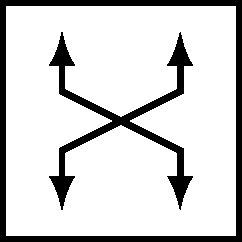
\includegraphics[width=0.9cm]{../common/fig-switch.pdf}
}
\providecommand{\router}{%
    
\includegraphics[width=0.9cm]{../common/fig-router.pdf}
}

\begin{frame}{network and switch tables}
\begin{tikzpicture}
\tikzset{
    computer/.style={inner sep=0mm,outer sep=0mm,execute at begin node={\computer}},
    switch/.style={inner sep=0mm,outer sep=0mm,execute at begin node={\switch}},
    connect/.style={draw,very thick,Latex-Latex},
    connect big/.style={draw,ultra thick,Latex-Latex},
    port/.style={pos=0.95,fill=white,circle,draw,inner sep=0mm},
    port beginning/.style={pos=0.05,fill=white,circle,draw,inner sep=0mm},
    mac label/.style={
        visible on=<2->,draw,fill=white,inner sep=1mm,font=\tiny\tt,
        alt=<2>{text=red,draw=red},
    },
    route table/.style={
        matrix of nodes,ampersand replacement=\&,
        column 1/.style={nodes={draw,thick,text width=2.5cm,font=\tiny\tt,text depth=0mm,minimum height=0.5cm,inner sep=1mm}},
        column 2/.style={nodes={draw,thick,text width=.5cm,font=\small\tt,text depth=0mm,minimum height=0.5cm,inner sep=1mm}},
        row 1/.style={nodes={draw=none,font=\small}},
    }
}
\foreach \x/\d/\mc/\dir in {15/8cm/AA/north,45/3cm/BB/north,90/2cm/CC/north,135/3cm/DD/north,180/4cm/EE/north,300/4cm/FF/south} {
    \node[computer,label={[mac label,]\dir:00:11:22:33:44:\small\mc}] (c-\x) at (\x:\d) {};
}
\node[switch,alt=<4>{fill=red!10}] (s1) at (4,-0.5) {};
\begin{visibleenv}<4->
\matrix[route table,alt=<4>{fill=red!10},anchor=north west] (s1 table) at ([xshift=1cm,yshift=.5cm]s1.north east) {
dst MAC addr \& port \\
00:11:22:33:44:\small AA \& 1 \\
00:11:22:33:44:\small BB \& 2 \\
00:11:22:33:44:\small CC \& 4 \\
00:11:22:33:44:\small DD \& 4 \\
00:11:22:33:44:\small EE \& 4 \\
00:11:22:33:44:\small FF \& 3 \\
};
\draw[dotted,thick] (s1.north east) -- (s1 table-2-1.north west);
\draw[dotted,thick] (s1.south east) -- (s1 table-7-1.south west);
\end{visibleenv}
\node[switch,alt=<3>{fill=red!10}] (s2) at (-1,0.5) {};
\begin{visibleenv}<3->
\matrix[route table,alt=<3>{fill=red!10},anchor=north east] (s2 table) at ([xshift=2cm]s2.south west) {
dst MAC addr \& port \\
00:11:22:33:44:\small AA \& 1 \\
00:11:22:33:44:\small BB \& 1 \\
00:11:22:33:44:\small CC \& 2 \\
00:11:22:33:44:\small DD \& 3 \\
00:11:22:33:44:\small EE \& 4 \\
00:11:22:33:44:\small FF \& 2 \\
};
\draw[dotted,thick] (s2.south east) -- (s2 table-2-2.north east);
\draw[dotted,thick] (s2.south west) -- (s2 table-2-1.north west);
\end{visibleenv}
\draw[connect] (c-15) -- (s1) node[port] {1};
\draw[connect] (c-45) -- (s1) node[port] {2};
\draw[connect] (c-300) -- (s1) node[port] {3};
\draw[connect] (c-90) -- (s2) node[port] {2};
\draw[connect] (c-135) -- (s2) node[port] {3};
\draw[connect] (c-180) -- (s2) node[port] {4};
\draw[connect big] (s1) -- (s2) node[port beginning] {4} node [port] {1};
\end{tikzpicture}
\end{frame}

\begin{frame}{constructing switch tables}
    \begin{itemize}
    \item could have system administrator input these by hand
        \begin{itemize}
        \item through an SSH-like interface, probably
        \end{itemize}
    \item works, but error-prone, hard to change, etc.
    \vspace{.5cm}
    \item<2-> alternative: switch should figure it out
    \end{itemize}
\end{frame}

\begin{frame}{MAC learning}
\begin{tikzpicture}
\tikzset{
    route table/.style={
        matrix of nodes,ampersand replacement=\&,
        column 1/.style={nodes={draw,thick,text width=2.5cm,font=\tiny\tt,text depth=1mm,text height=3.5mm,minimum height=0.6cm,inner sep=1mm}},
        column 2/.style={nodes={draw,thick,text width=1cm,font=\small\tt,text depth=1mm,text height=3.5mm,minimum height=0.6cm,inner sep=1mm}},
        row 1/.style={nodes={draw=none,font=\small}},
    }
}
\matrix[label={north:forwarding table},route table,draw,very thick,anchor=north east] (table) {
dst MAC addr \& port \\
|[alt={<5,7>{fill=red!10}}]| \alt<5->{00:11:22:33:44:AA}{~}
    \& |[alt={<5,7>{fill=red!10}}]| \alt<5->{2}{~} ~ \\
|[alt={<8>{fill=red!10}}]| \alt<8->{00:11:22:33:44:FF}{~}
    \& |[alt={<8>{fill=red!10}}]| \alt<8->{3}{~} ~ \\
~ \& ~ \\
~ \& ~ \\
~ \& ~ \\
~ \& ~ \\
|[alt={<2,4>{fill=red!10}}]|  \alt<2->{(default)}{~} 
    \& |[alt={<2,4>{fill=red!10}}]| \alt<2->{ALL*}{~} \\
};
\begin{visibleenv}<3->
\matrix[
    draw,very thick,label={north:incoming frame 1},anchor=north west,tight matrix,
    nodes={text width=8cm,font=\small}
] (pkt 1) at ([xshift=1cm]table.north east) {
    input port=\myemph<5>{2}, output port = \alt<4->{\myemph<4>{all but 2}}{\myemph<3>{???}} \\
    data = {
\begin{tabular}{l}
src=\tt \myemph<5>{00:11:22:33:44:AA} \\ dst=\tt \myemph<2>{00:11:22:33:44:FF} \\
type = IPV4  \\ data = \tt33 45 43 42 \ldots \\
\end{tabular}
} \\
};
\end{visibleenv}
\begin{visibleenv}<6->
\matrix[
    draw,very thick,label={north:incoming frame 2},anchor=north west,tight matrix,
    nodes={text width=8cm,font=\small}
] (pkt 2) at ([yshift=-1cm]pkt 1.south west) {
    input port=\myemph<8>{3}, output port = \alt<7->{\myemph<7>{2}}{???} \\
    data = {
\begin{tabular}{l}
src=\tt \myemph<8>{00:11:22:33:44:FF} \\ dst=\tt \myemph<7>{00:11:22:33:44:AA} \\
type = IPV4  \\ data = \tt34 45 43 42 \ldots \\
\end{tabular}
} \\
};
\end{visibleenv}
\end{tikzpicture}
\end{frame}

% FIXME: picture of network with switch ports labeled
    % FIXME: picture of ideal mac_dst_exact tables for it

% ideal: table of MAC addresses
% note: multiple MAC addresses per port
    % assumption: no loops
% fallback: broadcast

\begin{frame}{fallback option}
    \begin{itemize}
    \item very low quality switch: \\
    send every frame to every \textit{other} port
    \vspace{.5cm}
    \item receivers will check destination
        \begin{itemize}
        \item check dates to history of unswitched (shared medium) ethernet
        \item sending to extra destinations just slow
        \end{itemize}
    \vspace{.5cm}
    \item as optimization: want to only send where interested
    \end{itemize}
\end{frame}



% FIXME: example of using tcpdump/etc. in implementation

\subsection{aside: no loops please}

\usetikzlibrary{arrows.meta,decorations.markings,patterns}

\providecommand{\computer}{%
    
\includegraphics[width=1cm]{../common/Noun_project_216.pdf}
}
\providecommand{\switch}{%
    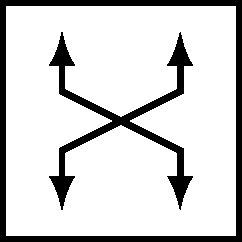
\includegraphics[width=0.9cm]{../common/fig-switch.pdf}
}
\providecommand{\router}{%
    
\includegraphics[width=0.9cm]{../common/fig-router.pdf}
}

\begin{frame}[label=noBackwardsQ]{aside: no backwards broadcast}
    \begin{itemize}
    \item recall: broadcast sent to all but incoming port
    \item question: what would happen if we didn't do this?
        \begin{itemize}
        \item multiple may apply
        \end{itemize}
    \end{itemize}
\begin{tabular}{l}
A. might cause host to receive duplicates \\
B. might cause copies sent to non-incoming port to be dropped \\
C. might cause frames sent at same time to be dropped \\
D. might cause frames sent much later to be dropped \\
\end{tabular}
\end{frame}

\begin{frame}[fragile]{loop from backwards broadcast}
\begin{tikzpicture}[remember picture]
\tikzset{
    computer/.style={inner sep=0mm,outer sep=0mm,execute at begin node={\computer}},
    switch/.style={inner sep=0mm,outer sep=0mm,execute at begin node={\switch}},
    connect/.style={draw,very thick,Latex-Latex},
    connect big/.style={draw,ultra thick,Latex-Latex},
    port/.style={pos=0.95,fill=white,circle,draw,inner sep=0mm},
    port beginning/.style={pos=0.05,fill=white,circle,draw,inner sep=0mm},
    mac label/.style={
        draw,fill=white,inner sep=1mm,font=\tiny\tt,
    },
    one packet/.style n args={3}{
        alt={<#1>{
            postaction=decorate,
            decoration={
                markings,
                mark={at position .5 with
                    \node[
                        thin,transform shape,draw,
                        preaction={fill=white},
                        pattern=crosshatch,pattern color=blue!50,font=\tt,#2
                    ]{#3};
                }
            }
        }},
    },
    one packet forward/.style 2 args={
        one packet={#1}{#2}{>>>},
    },
    one packet backward/.style 2 args={
        one packet={#1}{#2}{<<<},
    },
    hilite/.style={
        alt=<#1>{preaction={fill=red!20},pattern=none},
    },
}
\node[overlay,anchor=north east] at ([xshift=-1cm]current page.north east) {
    time step \myemph{\large\insertoverlaynumber}
};
\foreach \x/\d/\mc/\dir in {15/8cm/AA/north,45/3cm/BB/north,90/2cm/CC/north,135/3cm/DD/north,180/4cm/EE/north,300/4cm/FF/south} {
    \node[computer,label={[mac label,]\dir:00:11:22:33:44:\small\mc},alias=c-\mc] (c-\x) at (\x:\d) {};
}
\node[switch] (s1) at (4,-0.5) {};
\node[switch] (s2) at (-1,-2.5) {};
\draw[connect,one packet forward=1,one packet backward={2}{hilite=2}] (c-15) -- (s1) node[port] {1};
\draw[connect,one packet backward=2,one packet backward=4] (c-45) -- (s1) node[port] {2};
\draw[connect,one packet backward=2,one packet backward=4] (c-300) -- (s1) node[port] {3};
\draw[connect,one packet backward=3] (c-90) -- (s2) node[port] {2};
\draw[connect,one packet backward=3] (c-135) -- (s2) node[port] {3};
\draw[connect,one packet backward=3] (c-180) -- (s2) node[port] {4};
\draw[connect big,one packet forward=2,one packet backward={3}{hilite=3},one packet forward={4}{hilite=4}] (s1) -- (s2) node[port beginning] {4} node [port] {1};
\end{tikzpicture}
\end{frame}

\begin{frame}{loops}
    \begin{itemize}
    \item each packet keeps getting sent indefinitely
    \item remember: happens for \textit{every packet sent}
    \item quickly overwhelms link between switches
    \vspace{.5cm}
    \item but can just avoid by not sending back?
    \end{itemize}
\end{frame}

\begin{frame}[fragile]{loops with only-to-other}
\begin{tikzpicture}[remember picture]
\tikzset{
    computer/.style={inner sep=0mm,outer sep=0mm,execute at begin node={\computer}},
    switch/.style={inner sep=0mm,outer sep=0mm,execute at begin node={\switch}},
    connect/.style={draw,very thick,Latex-Latex},
    connect big/.style={draw,ultra thick,Latex-Latex},
    port/.style={pos=0.95,fill=white,circle,draw,inner sep=0mm},
    port beginning/.style={pos=0.05,fill=white,circle,draw,inner sep=0mm},
    mac label/.style={
        draw,fill=white,inner sep=1mm,font=\tiny\tt,
    },
    one packet/.style n args={3}{
        alt={<#1>{
            postaction=decorate,
            decoration={
                markings,
                mark={at position .5 with
                    \node[
                        thin,transform shape,draw,
                        preaction={fill=white},
                        pattern=crosshatch,pattern color=blue!50,font=\tt,#2
                    ]{#3};
                }
            }
        }},
    },
    two packet/.style n args={3}{
        alt={<#1>{
            postaction=decorate,
            decoration={
                markings,
                mark={at position .3 with
                    \node[
                        thin,transform shape,draw,
                        preaction={fill=white},
                        pattern=crosshatch,pattern color=blue!50,font=\tt,#2
                    ]{#3};
                },
                mark={at position .6 with
                    \node[
                        thin,transform shape,draw,dashed,
                        preaction={fill=white},
                        pattern=crosshatch,pattern color=blue!50,font=\tt,#2
                    ]{#3};
                }
            }
        }},
    },
    one packet forward/.style 2 args={
        one packet={#1}{#2}{>>>},
    },
    one packet backward/.style 2 args={
        one packet={#1}{#2}{<<<},
    },
    one packet both/.style 2 args={
        one packet={#1}{#2}{<</>>},
    },
    hilite/.style={
        alt=<#1>{preaction={fill=red!20},pattern=none},
    },
    hilite b/.style={
        alt=<#1>{dashed,preaction={fill=red!20},pattern=none},
    },
    hilite alt/.style={
        alt=<#1>{pattern=north west lines,pattern color=black!50},
    },
}
\node[overlay,anchor=north east] at ([xshift=-1cm]current page.north east) {
    time step \myemph{\large\insertoverlaynumber}
};
\foreach \x/\d/\mc/\dir in {15/8cm/AA/north,30/4cm/BB/north,90/2cm/CC/north,135/3cm/DD/north,180/4cm/EE/north,46/2cm/FF/north} {
    \node[computer,label={[mac label,]\dir:00:11:22:33:44:\small\mc},alias=c-\mc] (c-\x) at (\x:\d) {};
}
\node[switch] (s1) at (2.5,-0.5) {};
\node[switch] (s2) at (-1,-0.5) {};
\node[switch] (s3) at (6,-3.5) {};
\draw[connect,one packet forward=1,two packet={5}{}{<<<}] (c-15) -- (s3);
\draw[connect,one packet backward=2,two packet={5}{}{<<<}] (c-BB) -- (s3);
\draw[connect,one packet backward=3,
      one packet backward={4}{hilite alt=4},
      ] (c-FF) -- (s1);
\draw[connect,one packet backward=3,
      one packet backward={4}{hilite alt=4},
      ] (c-90) -- (s2);
\draw[connect,one packet backward=3,
      one packet backward={4}{hilite alt=4},
     ] (c-135) -- (s2);
\draw[connect,one packet backward=3,
      one packet backward={4}{hilite alt=4},
      ] (c-180) -- (s2);
\draw[connect big,one packet both={3}{hilite=3},] (s1) -- (s2);
\draw[connect big,one packet backward=2,one packet forward={4}{hilite b=4},
    one packet backward={5}{hilite=5}] (s1) -- (s3);
\draw[connect big,one packet backward={2}{hilite=2},
    one packet forward={4}{hilite=4},
    one packet backward={5}{hilite b=5}] (s2) -- (s3);
\end{tikzpicture}
\end{frame}



\section{preview: internetworks}

\begin{frame}{preview: routing}
    \begin{itemize}
    \item better ways to decide where to send packets
    \item \ldots but require coordinating between switches
        \begin{itemize}
        \item avoid loops
        \item choose between multiple paths
        \item avoid `flooding' for each new machine
        \end{itemize}
    \vspace{.5cm}
    \item problem also very important for large networks\ldots
    \item \ldots like the Internet
    \item we will revisit it when we talk about IP routing
    \end{itemize}
\end{frame}


\section{backup slides}
\begin{frame}\frametitle{backup slides}
\end{frame}

\section{switched networks}

\usetikzlibrary{arrows.meta,calc,shapes}
\providecommand{\computer}{%
    
\includegraphics[width=1cm]{../common/Noun_project_216.pdf}
}
\providecommand{\switch}{%
    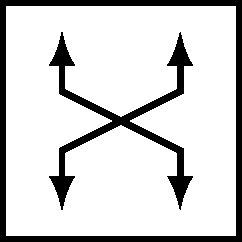
\includegraphics[width=0.9cm]{../common/fig-switch.pdf}
}
\providecommand{\router}{%
    
\includegraphics[width=0.9cm]{../common/fig-router.pdf}
}

\begin{frame}{recall: multi-access media}
\begin{tikzpicture}
\tikzset{
    connect/.style={draw,very thick,arrows={Latex-Circle[width=0.3cm,length=0.3cm]},
        alt=<2>{arrows={Latex-Circle[width=0.3cm,length=0.3cm,red]}}},
    computer/.style={inner sep=0mm,outer sep=0mm,execute at begin node={\computer}},
}
\draw[line width=1mm] (-5,-1.5) coordinate (wire start) -- (5, 1.5) coordinate (wire end);
\foreach \x/\d in {0/5cm,45/4cm,90/3cm,135/4cm,180/5cm,225/4cm,270/3cm,315/4cm} {
    \node[computer] (c-\x) at (\x:\d) {};
    \coordinate (connect-\x) at ($(wire start)!(c-\x.center)!(wire end)$);
    \draw[connect] (c-\x) -- (connect-\x) -- ([turn]0:.1cm);
}
\begin{visibleenv}<2-3>
\node[anchor=north west,fill=white,draw=black,thick,label={[font=\tiny]south:Ali at gwc.org.uk / Alistair1978 via Wikimedia commons / CC-BY-SA 2.5}] 
    (thicknet) at (4, 3.5) {
    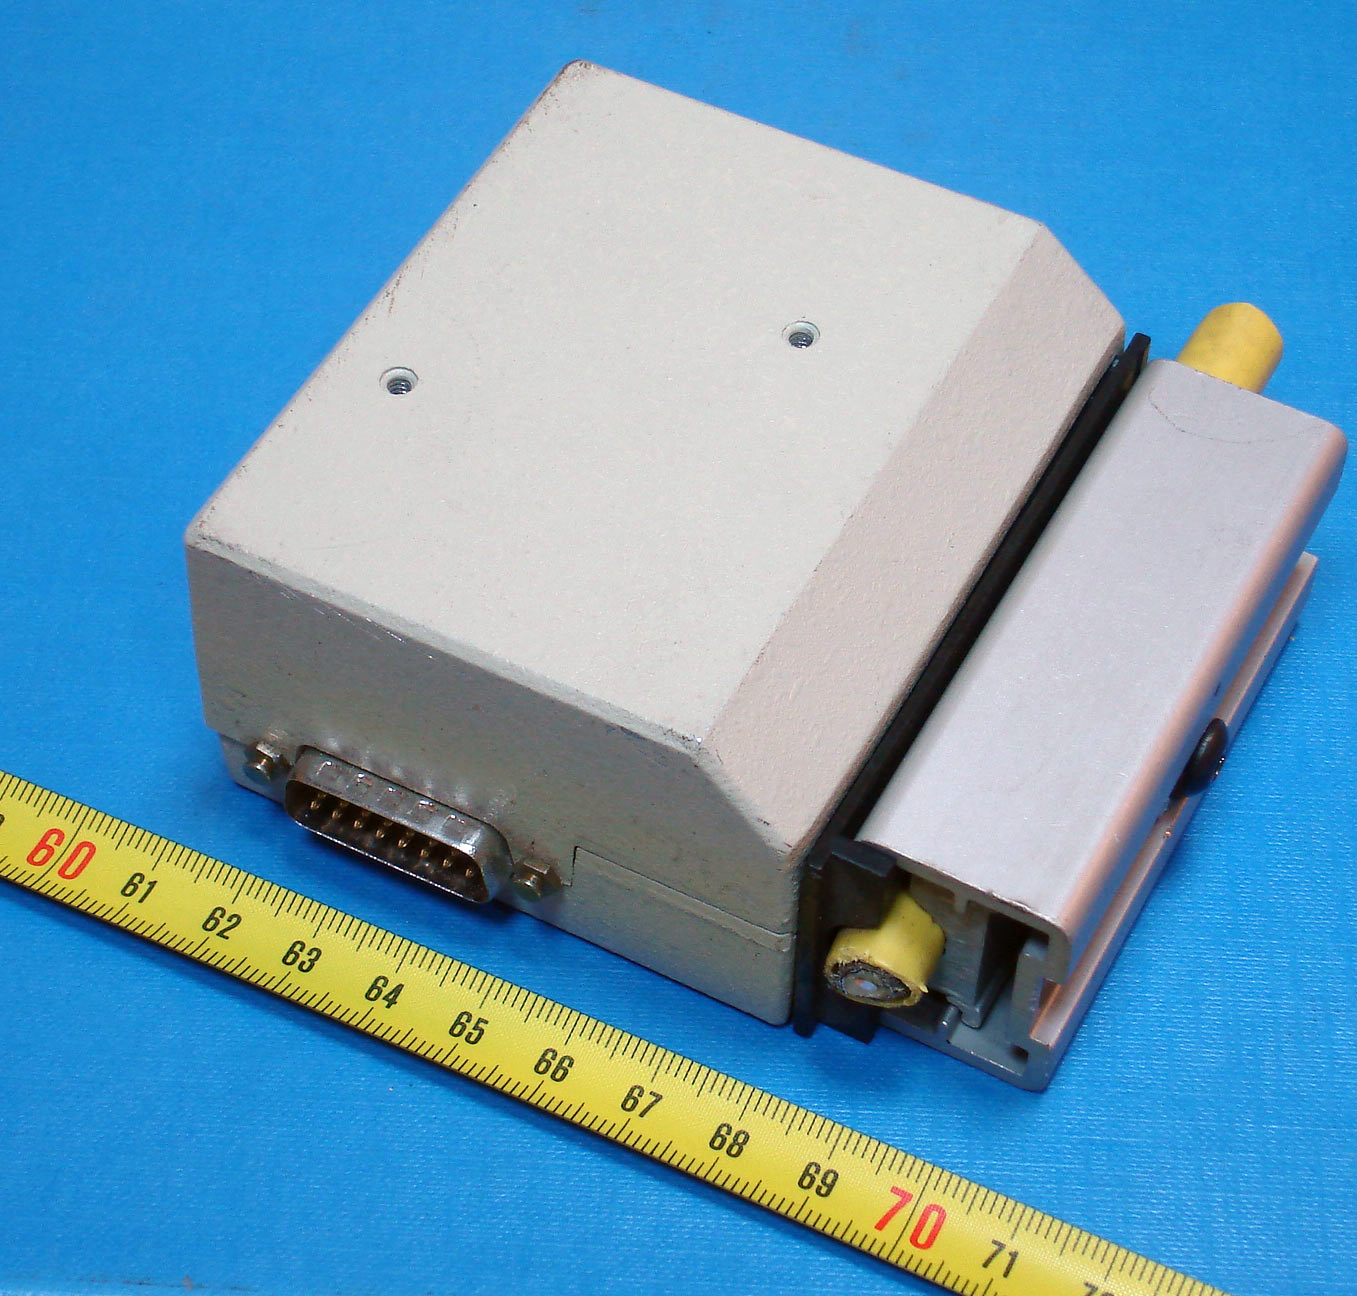
\includegraphics[width=4cm]{../intro/ThicknetTransceiver.jpeg}
};
\end{visibleenv}
\begin{visibleenv}<3>
\node[fill=white,draw=black,thick,anchor=north west] at ([yshift=-0.75cm]thicknet.south west) {
    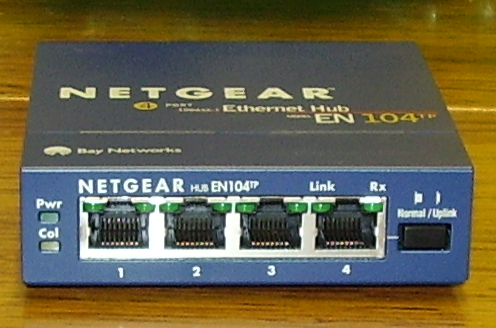
\includegraphics[width=4cm]{../intro/4_port_netgear_ethernet_hub}
};
% FIXME: also fiber splitter
\end{visibleenv}
\end{tikzpicture}
\end{frame}

\begin{frame}{recall: switched network}
\begin{tikzpicture}
\tikzset{
    computer/.style={inner sep=0mm,outer sep=0mm,execute at begin node={\computer}},
    switch/.style={inner sep=0mm,outer sep=0mm,execute at begin node={\switch},
                   alt=<1>{
                       fill=red!10,
                        label={[font=\small,label distance=0mm,text=red]south:`switch'}
                   }},
    connect/.style={draw,very thick,Latex-Latex,alt=<4>{red}},
    connect big/.style={draw,ultra thick,Latex-Latex,alt=<4>{red}},
}
\node[
      cloud,draw,opacity=0.25,very thick,aspect=2,
      minimum width=7cm,minimum height=4cm,
     ] (net-cloud) at (0,0) {};
\foreach \x/\d in {0/5cm,45/4cm,90/3cm,135/4cm,180/5cm,225/4cm,270/3cm,315/4cm} {
    \node[computer] (c-\x) at (\x:\d) {};
}
\node[switch] (s1) at (2,-0.5) {};
\node[switch] (s2) at (-1,0.5) {};
\node[switch] (s3) at (0,-1) {};
\draw[connect] (c-0) -- (s1);
\draw[connect] (c-45) -- (s1);
\draw[connect] (c-315) -- (s1);
\draw[connect] (c-90) -- (s2);
\draw[connect] (c-135) -- (s2);
\draw[connect] (c-180) -- (s2);
\draw[connect] (c-225) -- (s3);
\draw[connect] (c-270) -- (s3);
\draw[connect big] (s1) -- (s2);
\draw[connect big] (s1) -- (s3);
\coordinate (box loc) at (4cm, 4.5cm);
\end{tikzpicture}
\end{frame}

\begin{frame}{hubs and switches}
\begin{tikzpicture}
\node[fill=white,draw=black,thick,label={north:Hub}] (hub) {
    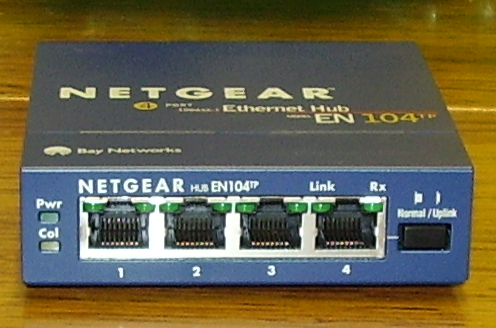
\includegraphics[width=6cm]{../intro/4_port_netgear_ethernet_hub}
};
\node[fill=white,draw=black,thick,anchor=north east,label={north:Switch}] (switch)  at (hub.north west){
    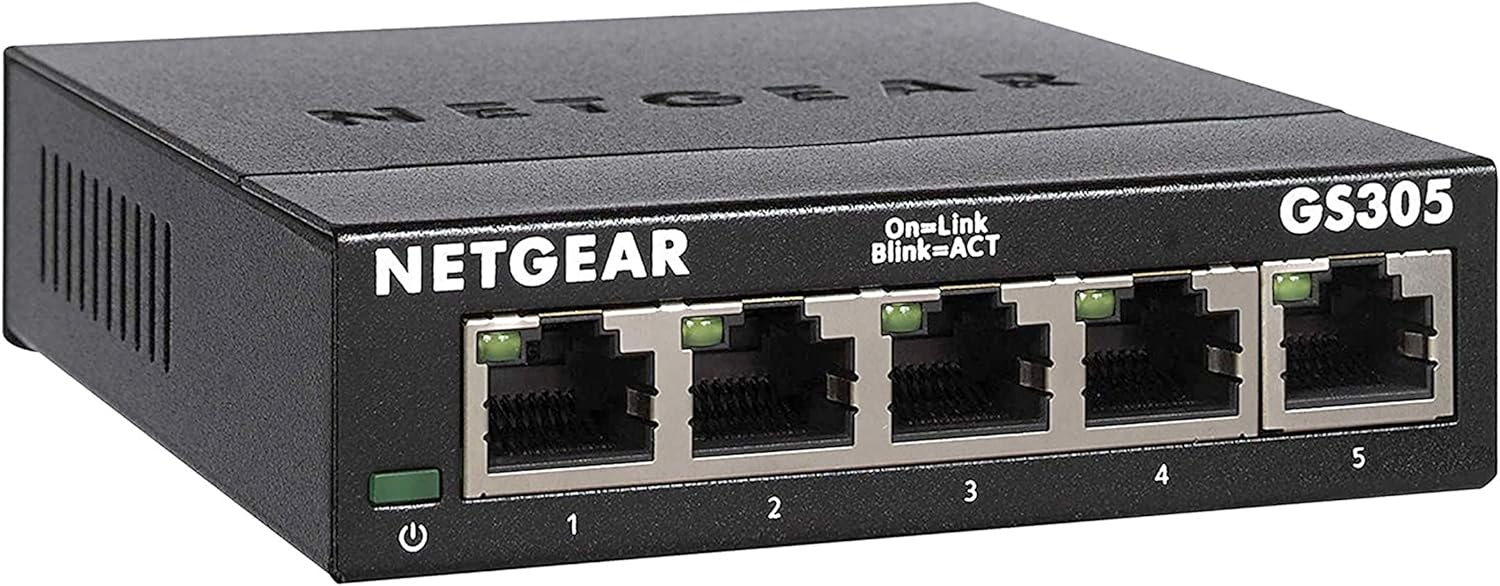
\includegraphics[width=6cm]{../switches/ModernNetgearSwitch}
};
\end{tikzpicture}
\begin{itemize}
\item difference is hidden inside
\item hub: electrically connects hosts --- as if shared wires
\item switch: decides what to send on each output
\end{itemize}
\end{frame}

\begin{frame}{history: multi-access to switched}
    \begin{itemize}
    \item a lot of early networking technology was multi-access
    \item wireless (wifi, cellular) and most home broadband still is
    \vspace{.5cm}
    \item most wired networks are \textit{switched}
        \begin{itemize}
        \item frames mostly directed to correct machine
        \end{itemize}
    \end{itemize}
\end{frame}

\begin{frame}{switching versus routing}
    \begin{itemize}
    \item switches --- forward frames for common network
    \item routers --- forward packets between networks
    \vspace{.5cm}
    \item basically same functionality
    \item differences:
        \begin{itemize}
        \item extra layer for internetwork packets
        \item different mechanism to decide where to forward
        \item switch forwarding typically simpler
        \end{itemize}
    \item will start with simpler switching
    \end{itemize}
\end{frame}


\end{document}
